\section{Xallary: Laborbeispielapp}
Für das bessere Verständis, zeigen von Features und zum einarbeiten in Xamarin haben wir eine App geschrieben, die 
momentan \textbf{unter Android} kompiliert wird, geschrieben.
In dieser App werden die Zugriffe auf die Kamera, auf den Lokalen- und Externenspeicher
gezeigt und wie ein Custom Element geschrieben wird, welches eine feste Android
Implementation ist, da hierbei auf Hardware- und API-Komponenten zugegriffen werden,
die Android spezifisch sind.
\subsection{Aufbau}
Eine Xamarin Applikation hat \textbf{immer} eine feste Grundstruktur, die aus drei Grundprojekten besteht.
Es können natürlich auch weitere Projekte hinzugefügt werden, aber es müssen immer folgende Projekte
vorhanden sein:
\begin{itemize}
    \item Klassenbibliothek
    \item Android, falls nur IOS dann wird das nicht benötigt
    \item IOS, falls nur Android wird dieses nicht benötigt
    \item UWP, dieses Projekt wird benötigt, wenn für Windowsgeräte entwickelt wird. Wie auch bei IOS und Android kann es, falls nicht benötigt, entfertn/deaktiviert werden.
\end{itemize}
(Figure \ref{fig:Ordnerstruktur}) 
\paragraph{Klassenbiliothek} Die Klassebibliothek ist nachdem Projekt benannt. 
Hier also Xallary. Wenn Crossplattformimplementationen 
getätigt werden, was die stärke von Xamarin ist, 
muss das hier geschehen,
da alle Projekte dieses als \textit{Dependency} haben. 
Das einzige, was hier nicht rein sollte und darf, sind Geräte/Betriebssystemabhängige Implementationen, da diese in den anderen Projekten erfolgen müssen.
\paragraph{Android} Sollen Android spezifische Implementationen vorgenommen werden, wie Beispielsweise \textit{Snackbars oder Toasts}, dann 
müssen diese in diesem Projekte implementiert werden. Außerdem muss bei nur androidspezisischen Hardwarekomponenten
diese hier per API Zugriffe implementiert werden. Zumteil sind aber schon Implementation in Xamarin behinhaltet und somit muss dann "nur"
diese in dem Projekt "angemeldet" werden.
\paragraph{IOS} Wie oben bei Android beschrieben, gilt auch hier dass spezfische \textit{OS} Implementation hier vollzogen werden müssen.
\begin{figure}[h]
    \centering
    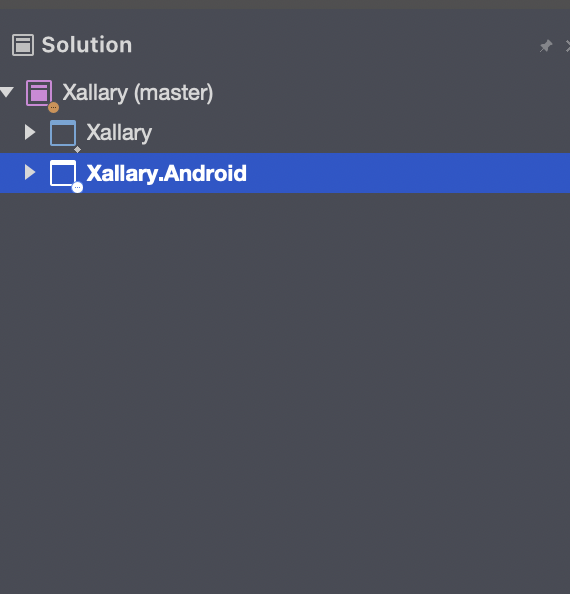
\includegraphics[width=0.9\textwidth]{Bildschirmfoto 2021-05-22 um 23.54.49.png}
    \label{fig:Ordnerstruktur}
    \caption{Orderstruktur von Xallary}
\end{figure}
\subsubsection{Verwendetes Designpattern}
Bei den Designpattern werden verschiedene in diesem Projekt verwendet. 

Zum einen wird das 
\textit{Dependency Injection Pattern} von \textit{Xamarin} verwendet, welches sich um die Verfügbarkeit von Klassen innerhalb
der Unterschiedlichen Projekten kümmert. Das Pattern übernimmt die Verwaltung der Klassen, ob diese bswp. als Singelton implementiert werden soll oder
die Initialisierung und Iinstanziierung.

Als weiteres Pattern wird das \textit{MVVM-Pattern}, also Model-ViewModel-View, verwendet.
Dieses Pattern ist ein sehr gängiges in der Welt von C\# beziehungsweise von WPF,UWP oder generell Frameworks welches \textit{Xaml} als 
\textit{MarkUpLanugage} verwenden.

Außerdem wird das \textit{Command Pattern} verwendet, welches dafür sorgt, dass die \textit{UI} keinen Code
in der \textit{Code Behind Datei}
\subsection{Permissionverwaltung}
%wo bzw wie können diese gesetzt werden 
%(MainActivity mit check, rechtklick auf das Projekt etc)

\subsection{Customelemente}
\subsubsection{Was sind \textit{Customelemente}}
\subsubsection{Implementation eines Customelementes für Android}
\subsubsection{App im Emulator/Smartphone}